\section{driver}
The Panstamps' drivers were developed in C++. Each member in the network, namely serverNode, actuatorNode and sensorNode, has its own driver; nevertheless, all of them are based on the class "node" as shown by the UML graph in Figure~\ref{fig:driverUML}. In other other words, ccServer, ccActuatorNode and ccSensorNode are all subclasses of the superclass "ccNode". 

All the nodes classes' names start with "cc" to denote that their communication depends completely on the class CC1101, which manages the CC1101 transceiver integrated in each Panstamp.

\begin{figure}[h!] 
 \centering
 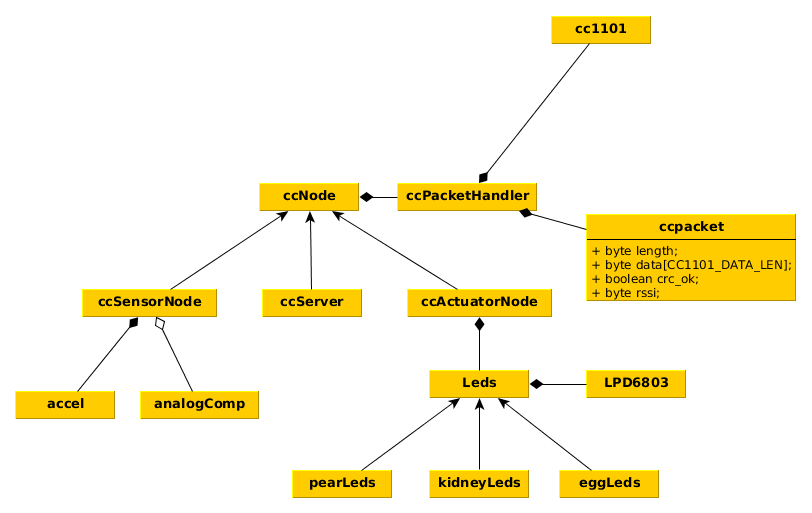
\includegraphics[width= 0.5\textwidth, clip=true,keepaspectratio=true]
 {./graph/driver_short.png}
 \caption{Driver's short UML }
 \label{fig:driverUML}
\end{figure}  

The class ccpacket contains the backbone for all the messages (packages) shared by the network's nodes. As depicted in Figure~\ref{fig:driverUML}, this class' attributes are:
\begin{itemize}
\item length, which determines the size of each package
\item data, an array that holds the packet information
\item crc\_ok. This boolean value set by the transceiver, upon receiving a packet, indicates the packet's data integrity. 
\item rssi. This value is set by the CC1101 that receives the packet and indicates the received signal strength.
\end{itemize}


\subsection{Packet's data array}
In our implementation, the packet's length was set to 6 bytes. There are two types of packets:
\begin{itemize}
\item Notification packets
\item Command packets
\end{itemize}

\subsubsection{Notification packet}
\label{sec:Notification packet}
Notification packets can be sent by all nodes of the network; they inform other nodes about current events. 
For example, when a node is moved or kicked, it broadcasts a notification packet to all nodes to inform about this occurrence. 

Table~\ref{Notification-packet} shows Notification packet's structure:

\begin{table}[h]
  \centering
  \begin{tabular}{ c | c }
    \hline
    \textbf{Name} & \textbf{Value}\\ [0.5ex]    
    \hline
    Receiver Id & data[0] \\
    Sender Id & data[1] \\
    Admin Key & data[2]\\
    Near Node Id or Dummy & data[3]\\
    Dummy & data[4]\\ 
    Checksum & data[5]\\		 
    \hline
  \end{tabular}
  \caption[Notification packet]%
          {Notification packet}
  \label{Notification-packet}
\end{table}

Depending on the value of "Receiver Id", a message is received by all nodes or just by a single one. To broadcast, "Receiver Id" has to be set to "0" (zero). In other words, a packet is broadcasted when packet.data[0] is set to "0" (see \url{http://code.google.com/p/panstamp/wiki/LowLevelLibrary}).
When the packet has to be sent to just a single node, "Receiver id" holds the receiver node id.

The "Sender Id" indicates which node created and sent the packet. This data is important for interpreting any packet's meaning.

"Admin Key" points out an specific event perceived by a node in the network. When a notification packet is received by the server, this node creates a new Panstamp-to-Java server message (see section~\ref{sec:Panstamp-to-Java server message}) to inform the Java server about the new event. Notification packets share the same keys as the Panstamp-to-Java server messages; to see all possible values that "Admin Key" can take, please refer to Table~\ref{Admin Keys}. 

When a module is moved or kicked, its sensor node broadcasts a notification packet (with "Admin Key" equal to \emph{shake\_event} or to \emph{kick\_event}) that is received by the all sensor nodes and by the server node. Each sensor node compares the rssi of the received notification packet to a specific threshold to determine if the node that broadcasted the notification packet is near. When the rssi is strong enough, the sensor node sends a notification packet to the server node with "Admin Key" equal to \emph{Near\_Node\_Event}. In this Notification packet, data[3] contains the id of the sensor node that was detected to be near. For the rest of the Notification packets, data[3] doesn't contain any real data (is a dummy value). 

To keep the same length for all packets, the Notification packets has a dummy byte in his data array ("data[4]"). Nevertheless, this data byte contains real data in the Command packets. 

"Checksum" stores the sum of all previous bytes in the data array (modulo 255). This byte is used as an additional indicator of the packet's integrity. Upon receiving a packet, the receiver node calculates the sum of the data array bytes (from data[0] to data[4]) modulo 256 and compares the result to the value stored in data[5] ("Checksum"). If the two values are not equal, the packet is considered to be corrupted; as a result, the packet is discarded.

\subsubsection{Command packets}
Command packets are sent only by the server node to the actuator nodes. 	

Table~\ref{Command-packet} shows the Command packet structure: 

\begin{table}[h]
  \centering
  \begin{tabular}{ c | c }
    \hline
    \textbf{Name} & \textbf{Value}\\ [0.5ex]    
    \hline
    Receiver Id & data[0] \\
    Sender Id & data[1] \\
    Metakey & data[2]\\
    Color1  & data[3]\\
    Color2 & data[4]\\ 
    Checksum & data[5]\\		 
    \hline
  \end{tabular}
  \caption[Command packet]%
          {Command packet}
  \label{Command-packet}
\end{table}

The two first fields, Receiver Id and Sender Id, are the same as the ones contained in the Notification packet section (see section~\ref{sec:Notification packet}). In a Command packet, the Sender Id byte will be always "1", the server Id, because only the server send Commands Packets.

"Metakey" indicates to the actuator node what pattern has to be displayed by the led strand. Table~\ref{Meta Keys} contains the patterns implemented in the system.

\begin{table}[h]
  \centering
  \begin{tabular}{ c | c }
    \hline
    \textbf{Name} & \textbf{Value}\\ [0.5ex]    
    \hline
    Blink & 0 \\
    Fade & 1 \\
    Rainbow & 2\\
    Leds On & 3\\
    Leds Off & 4\\ 
    Onestripe & 5\\
    Stripes & 6 \\
    \hline
  \end{tabular}
  \caption[Meta Keys]%
          {Meta Keys}
  \label{Meta Keys}
\end{table}

Most of the patterns displayed by the led strands has one or two colors. Fields "Color1" and "Color2" contain   keys that represent colors. The color pallet implemented in this system has 13 key colors but this pallet can be easily extended. 

As in the Notification packet, the last byte in the Command packet has a "Checksum", which is the sum of all previous bytes modulo 256 (see section~\ref{sec:Notification packet}). 

\subsection{ccPacketHandler}

The ccPacketHandler class is in charge of managing the creation, delivery and reception of packets in each node. For these tasks, this class employs the classes ccPacket and cc1101. 

\subsection{ccNode}
This abstract class is the base for all node classes.  
